%% ==============================
\chapter{\iflanguage{ngerman}{Konzept}{Technogical Fundations}}
\lstset { %
	language=C,
	backgroundcolor=\color{black!5}, % set backgroundcolor
	basicstyle=\footnotesize,% basic font setting
	breaklines=true,
	tabsize=3
}
\label{sec:Technogical Fundations}
%% ==============================
This chapter introduces technological foundations fundamental for the thesis, which includes methods, models and tools that are used later in the thesis. Section 3.1 focus on the basic principle of Unity3D, which is used to build simulation environment for generating synthetic images. Section 3.2 shortly explain the essential knowledge of deep learning, especially convolution neural network(CNN), which plays the basic role for our object detector. In Section 3.3 several deep neural network models with excellent performance in the field of computer vision are introduced.

\section{Unity3D background}
Unity3D\footnote{https://unity3d.com/de/unity} is a cross-platform game engine developed by Unity Technologies. Due to the motivation of transfer learning from sim to real, a simulation scene need to be built for generating large numbers of labeled image data. With Unity3D engine we are able to create virtual objects in 3D and render images based on scripting API in C\# . These features shows that Unity3D is suitable for our rendering requests and can simplify the works during modeling. 

\subsection{User interface}
Unity provides a basic graphical interface to build the simulation environment, which includes five basic windows. 
\begin{itemize}
	\item \textbf{The Scene View:} where user work with game objects, including models, lights and colliders, to construct the user's scenes. 
	\item \textbf{The Game View:} where user can preview and play simulation scene as a work in progress as user develop it.
	\item \textbf{The hierarchy window:} All of the game objects in the open scenes are listed by the hierarchy window in hierarchical order.
	\item \textbf{The project window:} where user imports, stores and edits the Asset files. 
	\item \textbf{The inspector window:} It is context sensitive and displays all the properties of any selected game object, asset or setting.
\end{itemize} 

The most common and useful windows of editor interface are shown in figure 3.1: 

\begin{figure}[h]
	\centering
	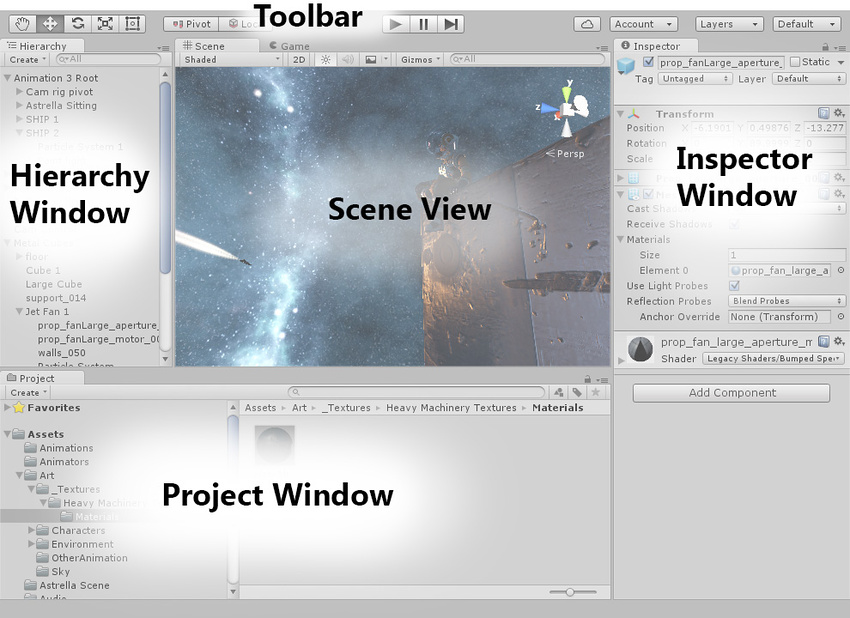
\includegraphics[width=0.8\textwidth]{Figures/Section3_Unity_interface}
	\caption{The most common and useful windows in Unity3D. The main editor window is made up of tabbed windows which can be rearranged, grouped, detached and docked. }
	\label{fig: unity interface}
\end{figure}

All the modeling works can be done in the graphical user interface. A general method of modeling are divided into 4 steps. Firstly a new default model needs to be created in Unity or imported from other 3D modeling software. This new model will appear in hierarchy window with other existent objects. Here the hierarchical relations can be adjusted. Secondly the dimensions and positions of new created model can be modified in inspector window, and new components (e.g. C\# scripts, Mesh Renderer, etc.) can be added into the model. Then in scene window a arbitrary perspective could be set, and according to the local coordinate system the position relationship among different objects can be adjusted. Finally when all items are correctly set and all needed components are added on them, the simulation scene can be played and the progress can be monitored in game view window in real time.

\subsection{Basic Concepts}

\subsubsection*{Coordinate System}

The world coordinate system is left handed (as Direct X) where x positive axis is right, y positive is up and z is positive into the screen, which is shown in figure 3.2.

\begin{figure}[h]
	\centering
	\begin{subfigure}{.6\textwidth}
		\centering
		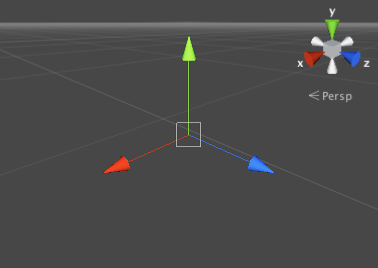
\includegraphics[width=\textwidth]{Figures/Section3_CoordinateSystem.png}
	\end{subfigure}
	\begin{subfigure}{.7\textwidth}
		\centering
		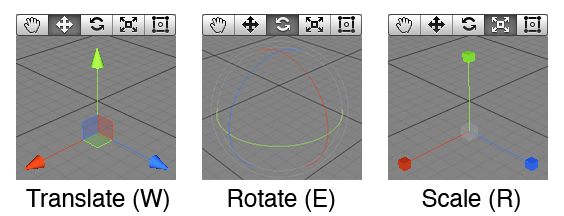
\includegraphics[width=\textwidth]{Figures/Section3_Transform}
	\end{subfigure}
	\caption{Coordinate system in Unity3D. Unlike the right-handed coordinate system in robotics, the left-hand coordinate system is used in Unity3D. }
	\label{fig: Coordinate unity}
\end{figure}

\begin{itemize}
	\item \textbf{Screen coordinate system} is bottom-up: (0,0) at bottom-left corner and (pixelWidth-1,pixelHeight-1) at right-top; x axis is positive right and y is positive up. The z position is in world units from the camera.
	\item \textbf{Viewport coordinate system} is normalized and relative to the camera, so the bottom-left point is (0,0), the top-right is (1,1). The z position is in world units from the camera.
	\item \textbf{UI coordinate system} is top-down: the y coordinate varies from zero at the top edge of the window to a maximum at the bottom edge of the window. The upper-left point is (0,0); the bottom-right is (1,1).
\end{itemize}


There are many functions to convert between all these different coordinate systems

\subsubsection*{Scene Construction}

To build a basic scene in Unity 3D, some important core concepts need to be discussed, including \textit{Game Object}, \textit{Component}, \textit{Script} and etc. They form the main basic elements of scene and various functions and effects can be realized with them. Normally, the \textit{Component} and \textit{Script} are sub-elements of the \textit{Game Object}.

\textbf{Scenes:} 

Scenes contain the objects of simulation project. They can be used to create a main menu, individual levels, and anything else. Each unique Scene file is a unique level. In each Scene, the environments, obstacles, decorations will be placed, and the project are designed and built in pieces.

A new Unity project will show a new Scene. The scene will be empty except for default objects- either an orthographic camera, or a  perspective camera and a directional light. An new empty scene is shown in figure 3.3.
\begin{figure}[h]
	\centering
	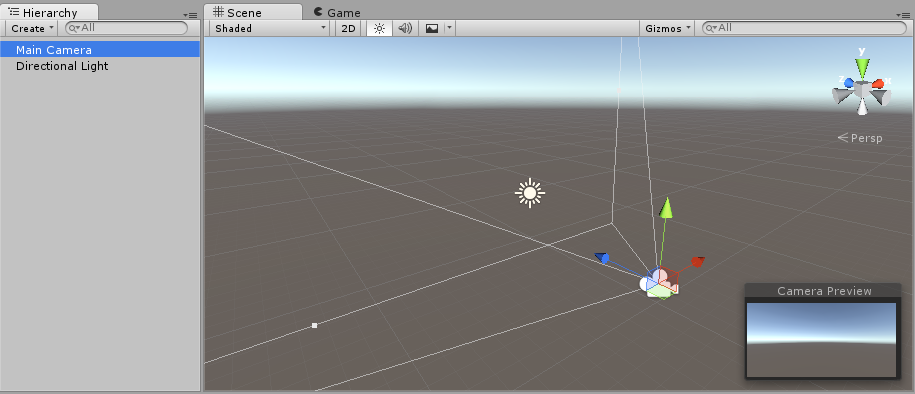
\includegraphics[width=0.8\textwidth]{Figures/Section3_NewEmptyScene}
	\caption{A new empty Scene, with the default 3D objects: a Main Camera and a directional Light.}
	\label{fig: new empty scene}
\end{figure}

\textbf{GameObjects:} 

The GameObject is the most important concept in the Unity Editor. Every object in project is a GameObject. This means that everything which can be thought of to be in the project has to be a GameObject. However, a GameObject can't do anything on its own; The properties need to be given before it can become a character, an environment, or a special effect.

A GameObject is a container; pieces are added to the GameObject container to make it into a character, a light, or whatever needed in project. Each added piece is called a component. Depending on what kind of object need to be created, different combinations of components can be added to a GameObject. A GameObject could be thought of as an empty cooking pot, and components are different ingredients that make up the recipe of project. 

\textbf{Component:} 

Components are the nuts \& bolts of objects and behaviors in a game. They are the functional pieces of every GameObject.

A GameObject is a container for many different Components. By default, all GameObjects automatically have a Transform Component. This is because the Transform dictates where the GameObject is located, and how it is rotated and scaled. Without a Transform Component, the GameObject wouldn't have a location in the word.

\textbf{Script: }

Scripting is an essential ingredient in all projects. They can be used to create graphical effects, control the physical behavior of objects and even implement a custom automatic system in the project. In next subsection, basic knowledge of scripting will be introduced to show how the script runs in unity and which basic functions are included in it. 


\subsection{Script Overview}
Unity3D supports the C\# programming language, which is an industry-standard language similar to Java or C++.

A script makes its connection with the internal workings of Unity by implementing a class which derives from the built-in class called MonoBehaviour. A class is like a kind of blueprint for creating a new Component type that can be attached to GameObjects. The core elements to realize different effects are the Event Functions. A script in Unity is not like the traditional idea of a program where the code runs continuously in a loop until it completes its task. Instead, Unity passes control to a script intermittently by calling certain functions that are declared within it. Once a function has finished executing, control is passed back to Unity. These functions are known as event functions since they are activated by Unity in response to events that occur during gameplay. Unity uses a naming scheme to identify which function to call for a particular event. There are four basic types of events as shown in figure 3.4:

\begin{figure}[h]
	\centering
	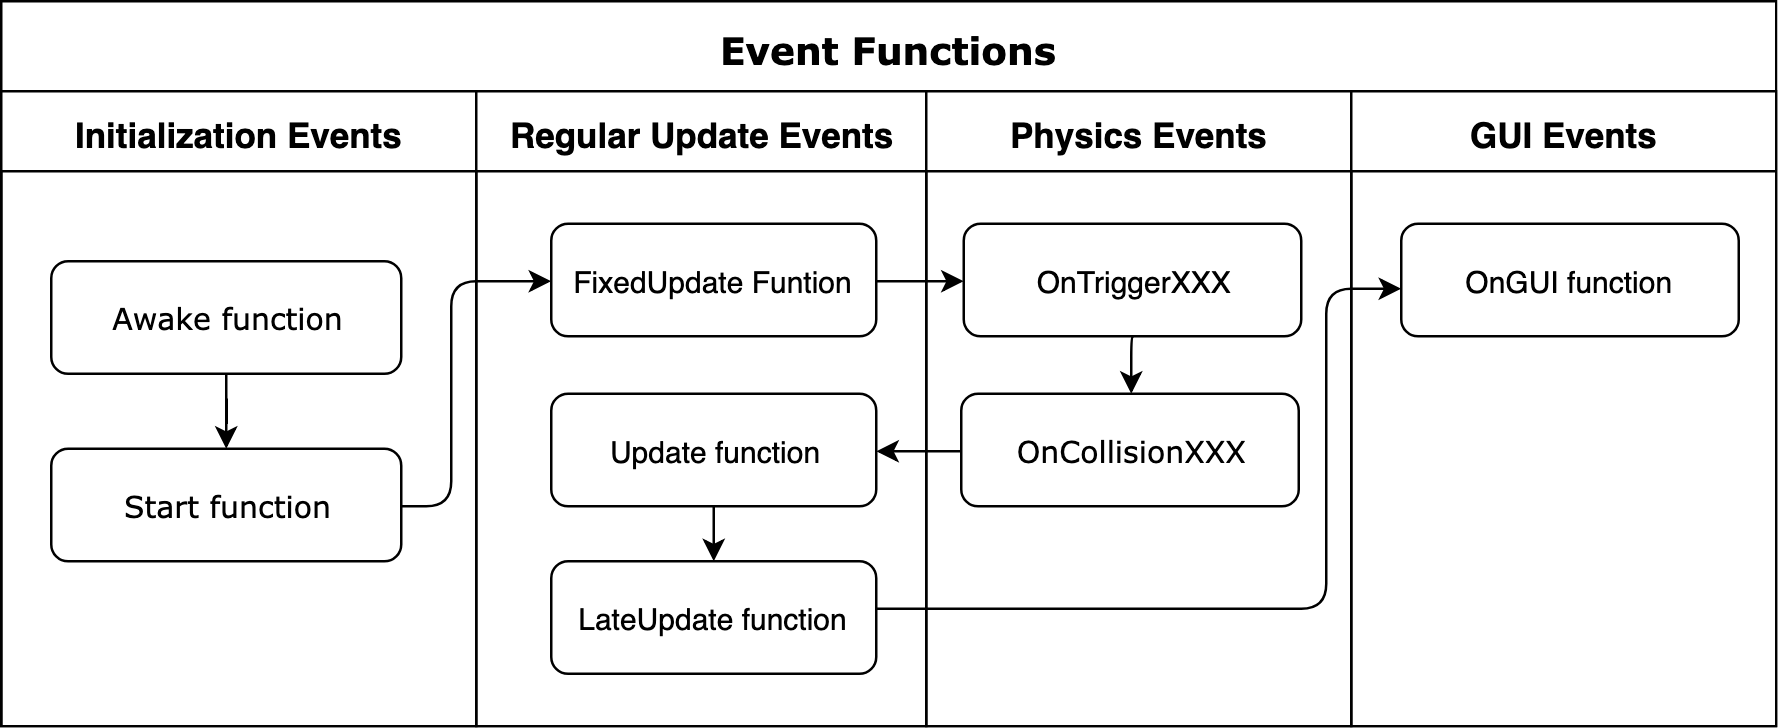
\includegraphics[width=\textwidth]{Figures/Section3_Eventfunction.png}
	\caption{Event function and execution order in Unity. For scene rendering, each event function is executed in order. Regular update and physics events execute in a loop, refresh the tasks in real-time}
	\label{fig: event_function}
\end{figure}



\subsubsection*{Regular Update Events: }
\begin{itemize}
	\item Update function: The Update function is the main place for making changes to position, state and behavior of objects in the scene just before each frame is rendered. Update is called before the frame is rendered and also before animations are calculated.
	\item FixedUpdate function: The physics engine also update in discrete time steps in a similar way to the frame rendering. A separate event function called FixedUpdate is called just before each physics update.
	\item LateUpdate function: It is also useful sometimes to be able to make additional changes at a point after the Update and FixedUpdate functions have been called for all objects in the scene and fter all animations have been calculated.
\end{itemize}

\begin{lstlisting}[caption=Regular Update Events Functions]
void Update() {
	float distance = speed * Time.deltaTime * Input.GetAxis("Horizontal");
	transform.Translate(Vector3.right * distance);
}

void FixedUpdate() {
	Vector3 force = transform.forward * driveForce * Input.GetAxis("Vertical");
	rigidbody.AddForce(force);
}

void LateUpdate() {
	Camera.main.transform.LookAt(target.transform);
}
\end{lstlisting}


\subsubsection*{Initialization Events:}
\begin{itemize}
	\item Start function: It is called before the first frame or physics update on an object.
	\item Awake function: The Awake function is called for each object in the scene at the time when the scene loads. All the Awakes will have finished before the first Start is called. This means that code in a Start function can make use of other initializations previously carried out in the Awake phase.
\end{itemize}


\subsubsection*{GUI event:} 
Unity has a system for rendering GUI controls over the main action in the scene and responding to clicks on these controls. This code is handled somewhat differently from the normal frame update and so it should be placed in the OnGUI function, which will be called periodically.

\begin{lstlisting}[caption=GUI  Events Functions]
void OnGUI() {
	GUI.Label(labelRect, "Game Over");
}
\end{lstlisting}


\subsubsection*{Physics events:} 
The physics engine will report collisions against an object by calling event functions on the object's script. 		
\begin{lstlisting}[caption=Physics Events Functions]
void OnCollisionEnter(otherObj: Collision) {
	if (otherObj.tag == "Arrow") {
	ApplyDamage(10);
	}
}
\end{lstlisting}



\section{Deep Learning and Convolutional Neural Network}
In this section a introduction to neural network and deep learning are presented with the aim of enabling the reader to build up a precise understanding of the concepts and ideas as well as of the thesis' context.

\subsection{Machine Learning}
Learning algorithms are widely used in computer vision applications. Before considering image related tasks, we are going to have a brief look at basics of machine learning.

Machine learning has emerged as a useful tool for modeling problems that are otherwise difficult to formulate exactly. Classical computer programs are explicitly programmed by hand to perform a task. With machine learning, some portion of the human contribution is replaced by a learning algorithm \cite{goodfellow2016deep}. As availability of computational capacity and data has increased, machine learning has become more and more practical over the years, to the point of being almost ubiquitous.

A practical view of a machine learning system is depicted in Figure 3.5. The process is split into two phases. In the first phase, the machine learning algorithm is used to learn from the training data, and the second phase is the prediction. The training data could be labeled images of vehicles with the task to predict the pose. The machine learning algorithm learns a model on these data and this model can then used to predict unseen images of the same task. This prediction is happen in the second phase and apply only the learned model. In our example, the learned model get images of a vehicle and must predict the pose.
\begin{figure}[h]
	\centering
	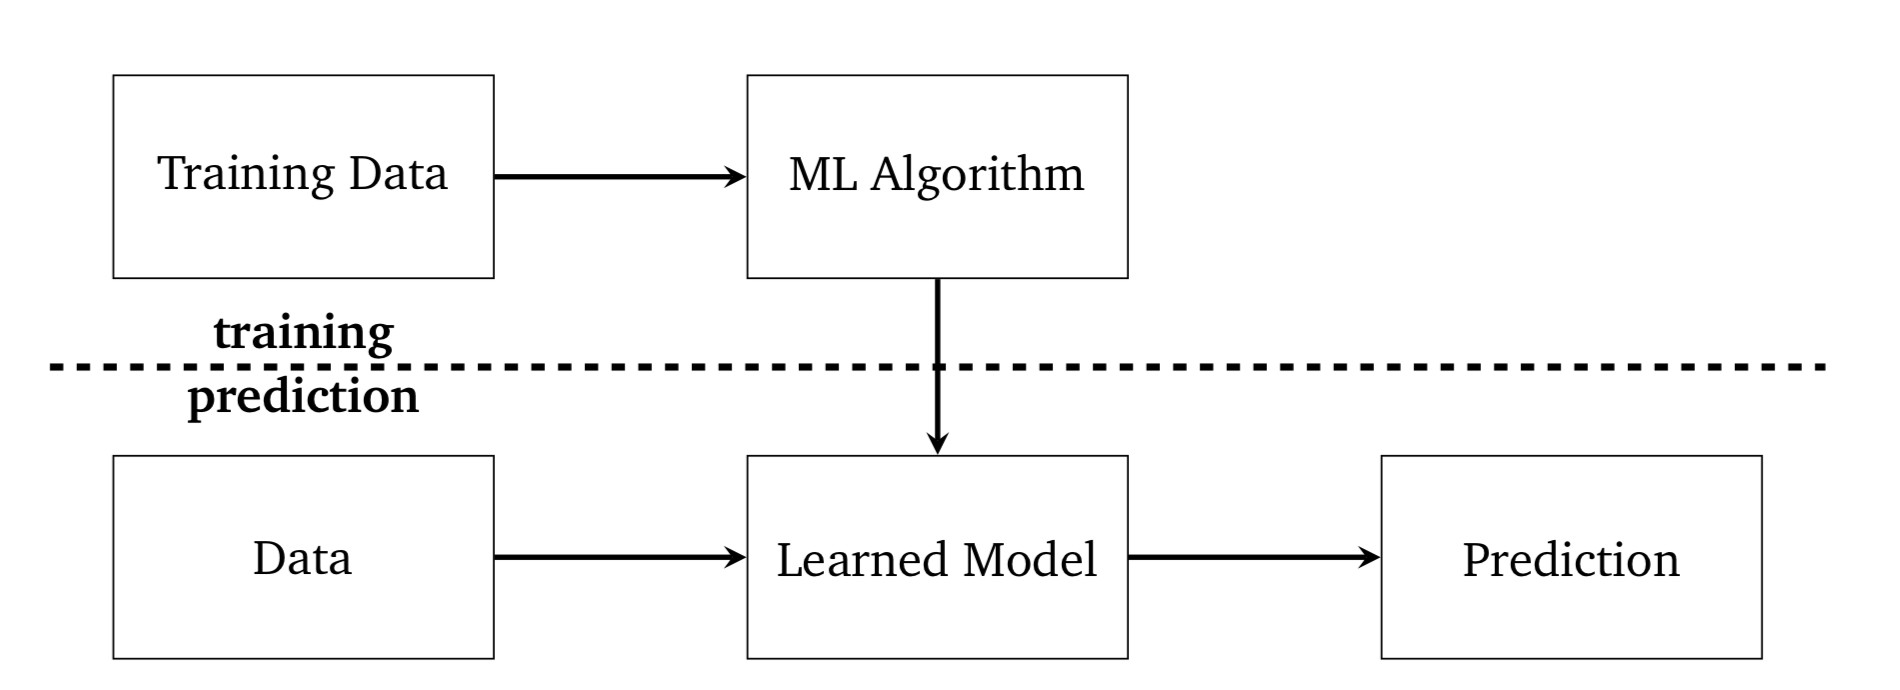
\includegraphics[width=\textwidth]{Figures/Section3_ML}
	\caption{Workflow of a machine learning problem. The data will be used to train a model with a machine learning algorithm. Then, in the prediction phase, the learned model can be used to generate a prediction.}
	\label{fig: machine learning}
\end{figure}

\subsubsection*{Types of Learning Problem}
In machine learning it can be distinguished between different learning problems. The main learning problems are:
\begin{itemize}
	\item \textbf{Supervised Learning:} A typical way of using machine learning is supervised learning \cite{bishop2006pattern}. A learning algorithm is shown multiple examples that have been annotated or labeled by humans. For example, in the object detection problem we use training images where humans have marked the locations and classes of relevant objects. After learning from the examples, the algorithm is able to predict the annotations or labels of previously unseen data. 
	\item \textbf{Unsupervised Learning:} In unsupervised learning, the algorithm attempts to learn useful properties of the data without a human teacher telling what the correct output should be. Classical example of unsupervised learning is clustering \cite{bishop2006pattern}. More recently, especially with the advent of deep learning technologies, unsupervised preprocessing has become a popular tool in supervised learning tasks for discovering useful representations of the data \cite{bengio2013representation}.
	\item \textbf{Reinforcement Learning:} In reinforcement learning the machine learning algorithm interact with an environment and must reach a certain goal. This could be to learn to playing a game, or to driving a vehicle in a simulation. The algorithm gets only information how good or bad he has interact with the environment. For example in learning to play a game, could this information the winning or losing of a game.
\end{itemize}

\subsubsection*{Types of Learning Tasks}
Classification and regression are the most important task types \cite{bishop2006pattern}. In classification, the algorithm attempts to predict the correct class of a new piece of data based on the training data. In regression, instead of discrete classes, the algorithm tries to predict a continuous output.

\begin{figure}[h]
	\centering
	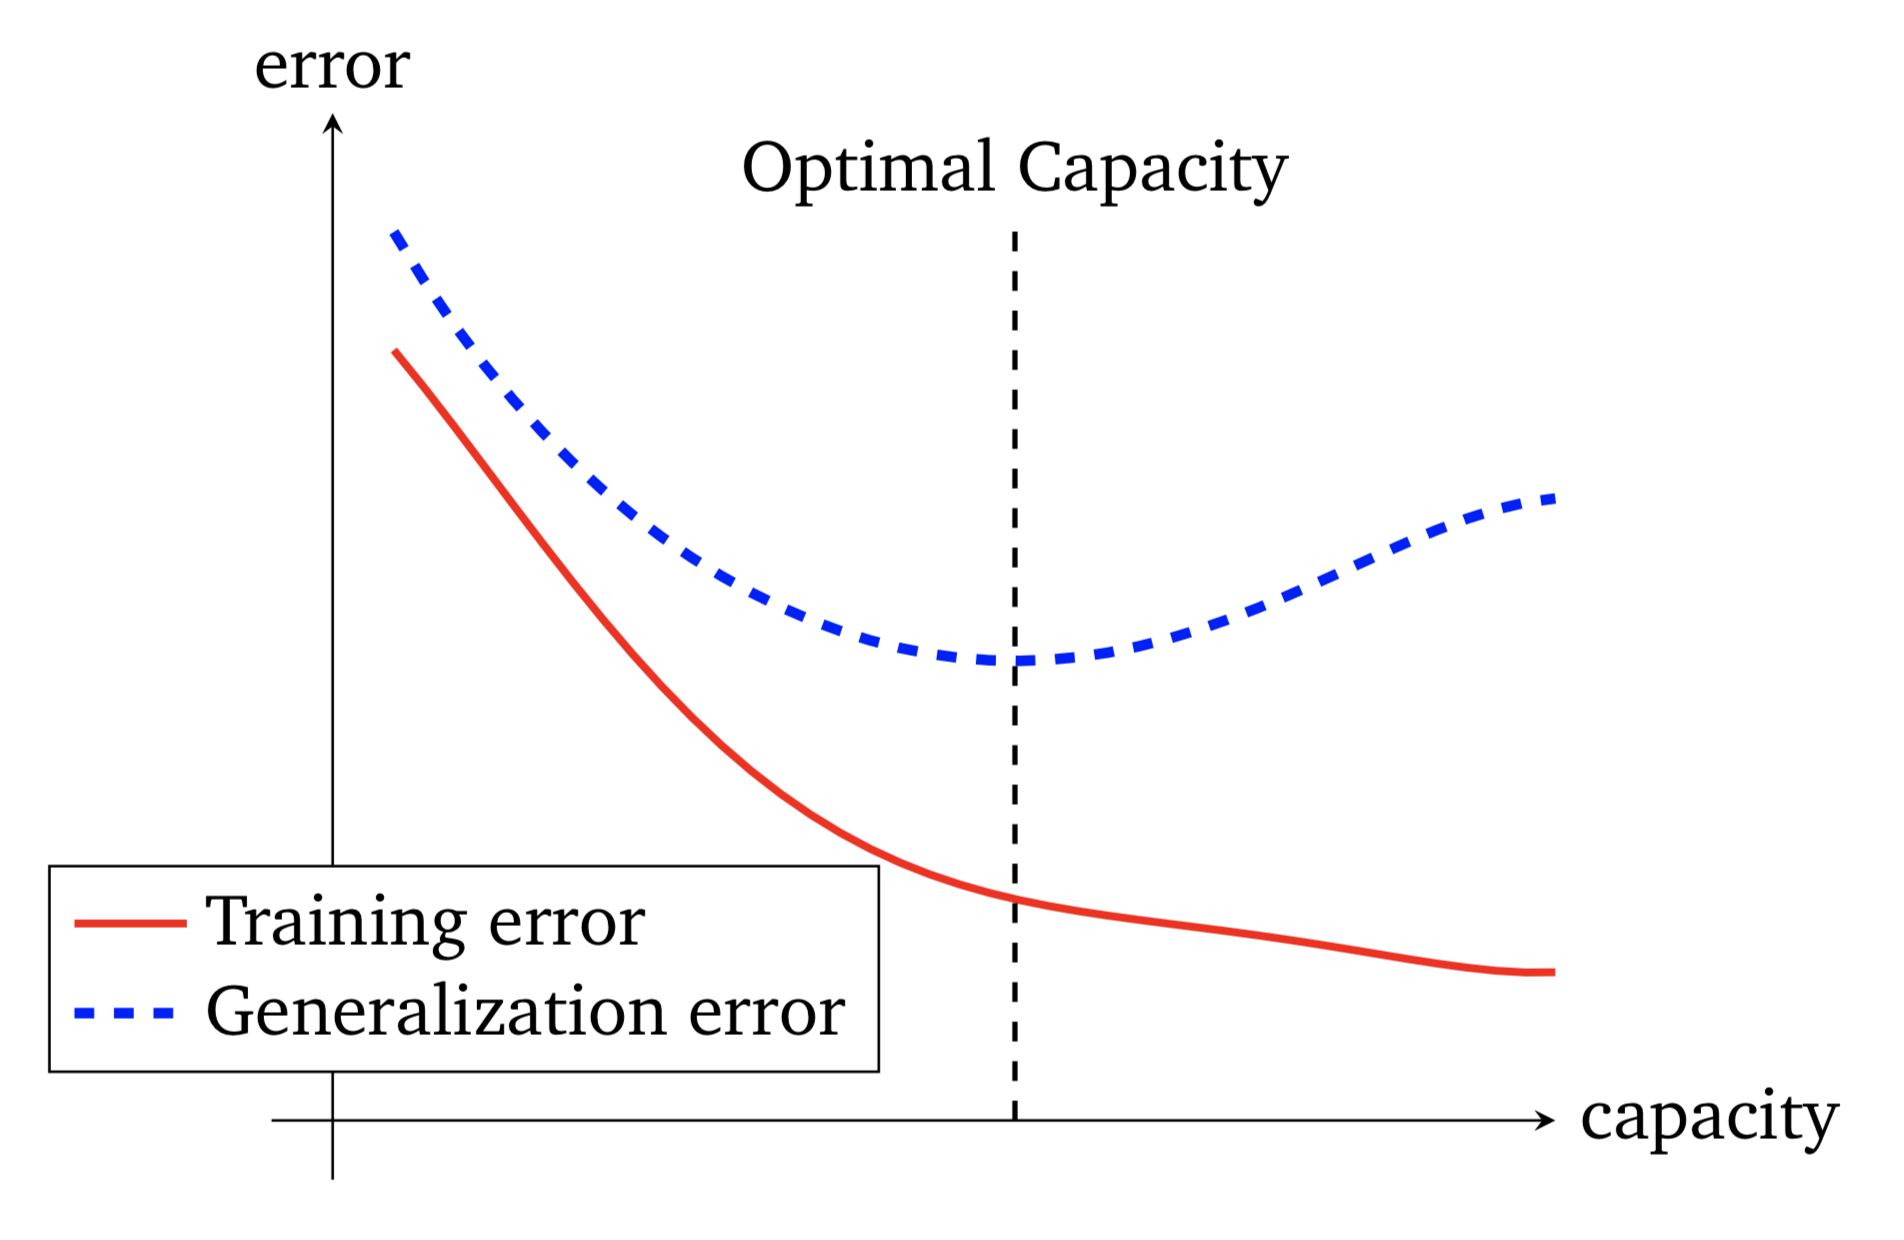
\includegraphics[width=0.8\textwidth]{Figures/Section3_Generalization}
	\caption{Shows typical curves for training and generalization error in dependency of the capacity of the model. Optimal capacity is reached at the minimal generalization error. Left of the optimal capacity is the model underfitting. On the right side of the optimal capacity is the model overfitting. The generalization error has typical a U-shaped curve.}
	\label{fig:  Generalization}
\end{figure}

\subsubsection*{Under- and Overfitting}
A machine learning algorithm must perform well on unseen data. The ability to perform well on unseen data is called generalization. The generalization error is measured on a test set. If a model perform not well on unseen data, then there are two reasons. Either the model has not enough capacity and underfit the underlying function, or it has too much capacity and overfit the underlying function. If a model is underfitting, then will be the training error and also the test error high. If the model is overfitting, then is the training error low and the test error high. The goal is to find a model, which has a low generalization error. The typical curves for training and generalization error are depicted in Figure 3.6.

In Figure 3.7 are three diagrams depicted, which shows the same noisy sampling of a sinus function. The samples are used learn a model, which describes the underlying function. The left diagram learned a model with a low capacity. So the training error is high and a test set would be also produce a high test error. In the center is depicted a model with a higher capacity. This shows a good approximation of the underlying function. Nevertheless the model has a training error, because we sampled the sinus with noise. But this model will have on a test set the best generalization error compared to the other two models. The third diagram shows a model with a high capacity. The training error will be low, but the learned model is not a good approximation of the sinus function, which would result on a test set with a high error.

\begin{figure}[h]
	\centering
	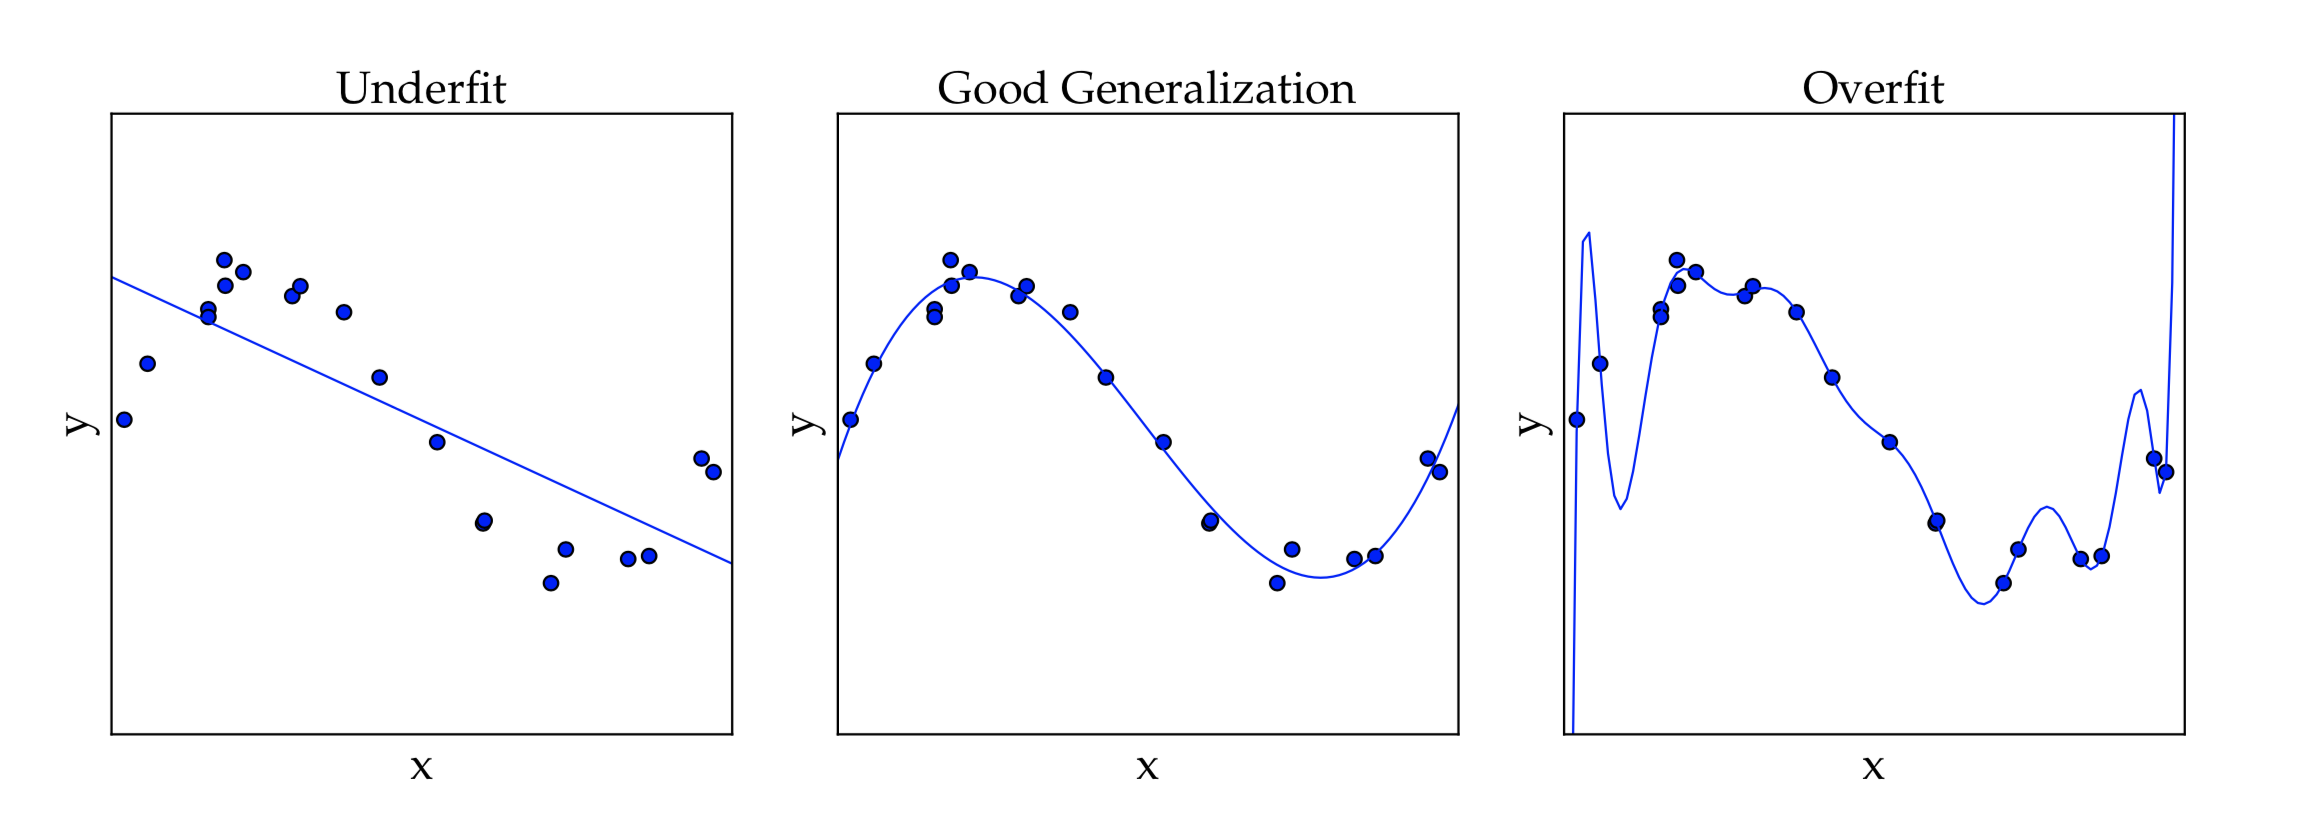
\includegraphics[width=0.8\textwidth]{Figures/Section3_Fitting}
	\caption{Theses three diagrams show three different models, which tries to fit the sampled points. The sampled points are sampled from a noisy sinus function. The models are described by a polynom of degree {1,4,15}. The left model underfits the underlying function. The model in the center is a good approximation of the underlying function. The right model overfits the underlying function. It has the smallest error to fit the sampled points, but on unseen samples, it will be provide a bad error \cite{goodfellow2016deep}.}
	\label{fig: fitting}
\end{figure}

\subsection{Neural Network Basis}
Neural networks are a popular type of machine learning model. A special case of a neural network called the convolutional neural network (CNN) is the primary focus of this thesis. Before discussing CNNs, we will discuss how regular neural networks work.

\subsubsection*{Biological Motivation and Neural Network Architecture}
The basic computational unit of the brain is a neuron. Approximately 86 billion neurons can be found in the human nervous system and they are connected with approximately $10^{14}$-$10^{15}$ synapses \cite{long2008scalable}. The diagram below shows a cartoon drawing of a biological neuron and a common mathematical model.

\begin{figure}[h]
	\centering
	\begin{subfigure}{0.8\textwidth}
		\centering
		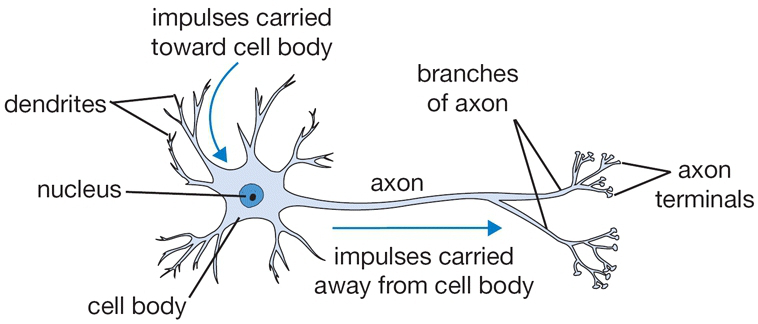
\includegraphics[width=0.9\linewidth]{Figures/Section3_NeuroStructure.png} 
	\end{subfigure}
	\begin{subfigure}{0.7\textwidth}
		\centering
		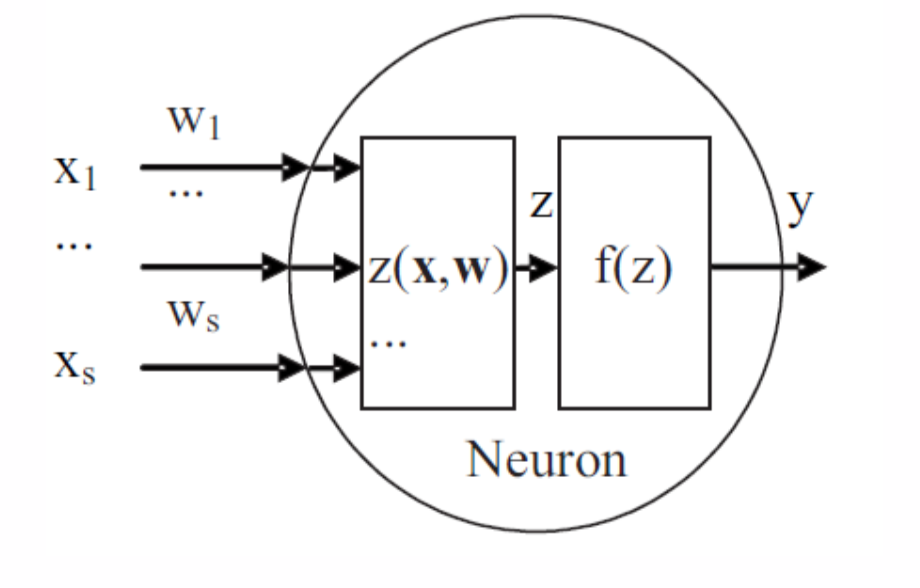
\includegraphics[width=0.7\linewidth]{Figures/Section3_OneNeuron_1.png} 
	\end{subfigure}
	\caption{a single Neuron example. At the top is the biological structure, and at the bottom is the simplified mathematical model.}
	\label{fig:unit of a neuron}
\end{figure}

An artificial neuron based on the McCulloch-Pitts model is shown in Figure 3.9 \cite{bishop2006pattern}. The neuron k receives m input parameters $ x_{i} $. The neuron also has m weight parameters $ W_{i} $. The weight parameters often include a bias term that has a matching dummy input with a fixed value of 1. The inputs and weights are linearly combined and summed. The sum is then fed to an activation function $ f $ that produces the output $ y $ of the neuron:
\begin{equation}
	y_{ k }=f\left( z_{ k } \right)=f\left( \sum_{ j=0 }^{s}{ w_{ kj }x_{ j } } \right)
\end{equation}
The above neuron composed of multiple elements, which have different features and play various role in the neuron networks. Besides the inputs and outputs, the weights and activation function are the most important parts, which decide the basic function of a neuron. The network consists of connections, each connection transferring the output of a neuron $i$ to the input of a neuron $j$. In this sense $i$ is the predecessor of $j$ and $j$ is the successor of $i$, each connection is assigned a weight $W_{ij}$

\subsubsection*{Activation Functions}
The activation function of a node defines the output of that node given an input or set of inputs. To approximate nonlinear function each neuron has to perform nonlinear transformation of its input, which is done with activation function $f(z)$. There are several different commonly used activation functions. Its usage depends on the type of network and also on the type of layer in which they operate. An example of different activation functions are shown in figure 3.9.

\begin{figure}[h]
	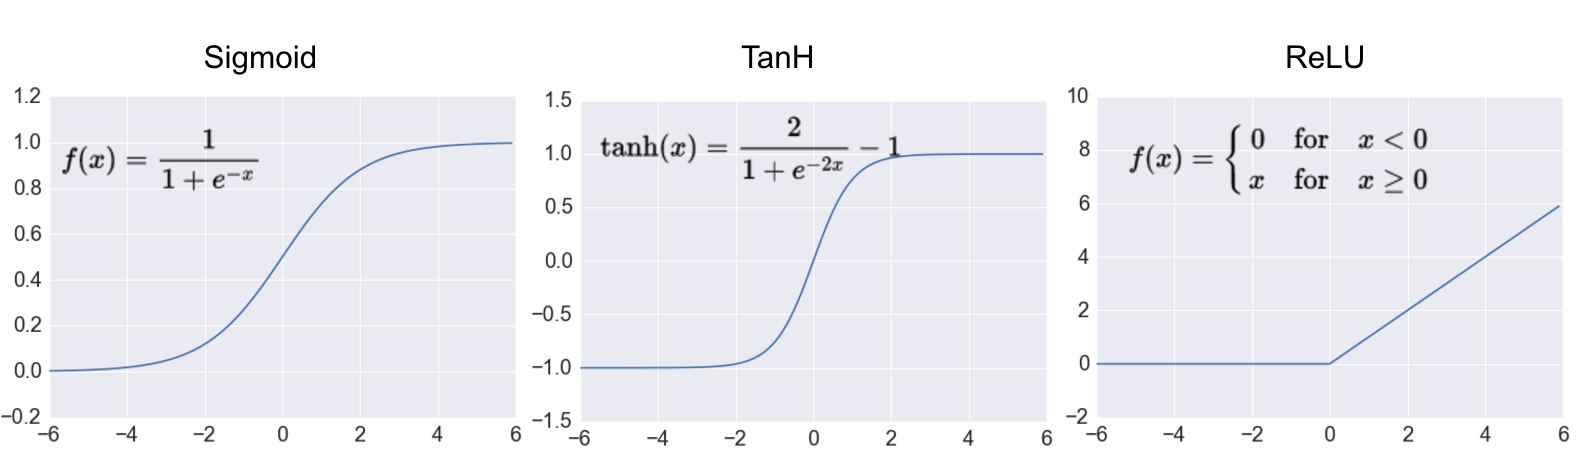
\includegraphics[width=\textwidth]{Figures/Section3_activation.png} 
	\captionsetup{justification=centering}
	\caption{Most popular activation functions: Sigmoid, Tanh, ReLU}
	\label{fig:activation}
\end{figure}
\begin{itemize}
	\item \textbf{Sigmoid:} One of the oldest and historically most commonly used activation function is sigmoid function. It is defined by
	\begin{equation}
	g(x)=\frac{1}{1+e^{-x}}
	\end{equation}
	It takes a real value and squashes it between 0 and 1. However, when the neuron’s activation
	saturates at either tail of 0 or 1, the gradient at these regions is almost zero. Thus, the backpropagation algorithm fail at modifying its parameters and the parameters of the preceding neural layers.
	
	\item \textbf{Hyperbolic Tangent:} The TanH non-linearity has the following mathematical form:
	\begin{equation}
	y=\tanh(-x)
	\end{equation}
	It squashes a real-valued number between -1 and 1. However it has the same drawback than the sigmoid.
	
	\item \textbf{Rectified Linear Unit:} The ReLU has the following mathematical form:
	\begin{equation}
	y=max{0,x}
	\end{equation}
	The ReLU has become very  popular in the last few years, because it was found to greatly accelerate the convergence of stochastic gradient descent compared to the sigmoid/tanh functions due to its linear non-saturating form \cite{krizhevsky2012imagenet}. In fact, it does not suffer from the vanishing or exploding gradient. An other advantage is that it involves cheap operations compared to the expensive exponentials. However, the ReLU removes all the negative information and thus appears no suited for all datasets and architectures.
	
	\item \textbf{Leaky RelU:} To enlarge the range of the ReLU in negative direction, Leaky ReLU uses a small slop(usually 0.01), hence the Leaky ReLU can tend to infinity in both directions:
	\begin{equation}
	y=\begin{cases} x & \text{if $x>0$}  \\
	ax & \text{otherweise}
	\end{cases}
	\end{equation}
	where $a$ is a small constant.	
\end{itemize}


\subsubsection*{Structure of a shallow Neural Network}
There are many classes of neural networks and these classes also have sub-classes, e.g. feedforward, lateral and feedback connections. Here the most used ones will be listed - Feedforward neural network, which is shown in figure 3.10.

\begin{figure}[h]
	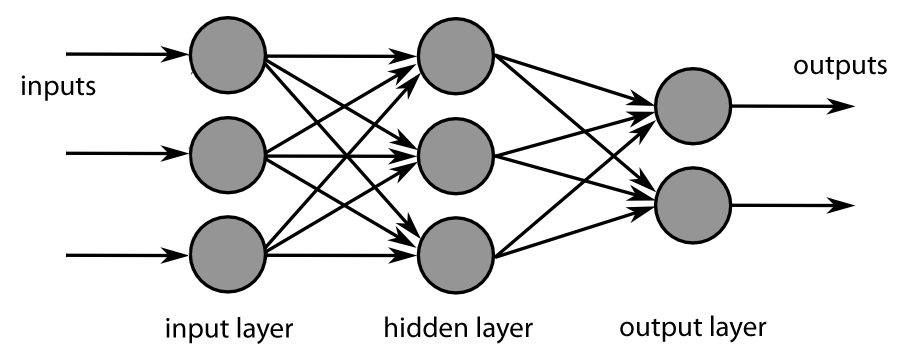
\includegraphics[width=\textwidth]{Figures/Section3_FeedforwardNN.png} 
	\captionsetup{justification=centering}
	\caption{A feedforward Multi-layer perceptron(MLP)}
	\label{fig:MLP}
\end{figure}

A feedforward neural network can consist of three types of layers:

\begin{itemize}
	\item \textbf{Input Layer:} No computation is done here within this layer, they just pass the information to the next layer (hidden layer most of the time).
	\item \textbf{Hidden Layer:} In Hidden layers is where intermediate processing or computation is done, they perform computations and then transfer the weights (signals or information) from the input layer to the following layer (another hidden layer or to the output layer). It is possible to have a neural network without a hidden layer, which is called Single layer Perceptron.
	\item \textbf{Output Layer:} Here an activation function can be used to maps to the desired output format (e.g. softmax for classification) .
\end{itemize}

The feedforward neural network was the simplest type of artificial neural network devised, where connections between the units do not form a cycle. In this network, the information moves in only one direction, forward, from the input nodes, through the hidden nodes (if any) and to the output nodes. 

\subsubsection*{Loss Functions and Optimization Problem}
Loss function is an important part in artificial neural networks, which is used to measure the inconsistency between predicted value  $ \hat{y} $and actual label $ y $. It is a non-negative value, where the robustness of model increases along with the decrease of the value of loss function. The aim of supervised learning is to minimize the overall cost, thus optimizing the correlation of the model to the system that it is attempting to represent. An optimization problem seeks to minimize a loss function. 

For the regression problem, several loss functions are commonly used:

\begin{itemize}
	\item \textbf{Mean Squared Error:} Mean Squared Error (MSE), or quadratic, loss function is widely used in linear regression as the performance measure, and the method of minimizing MSE is called Ordinary Least Squares (OSL), the basic principle of OSL is that the optimized fitting line should be a line which minimizes the sum of distance of each point to the regression line, i.e., minimizes the quadratic sum. The standard form of MSE loss function is defined as:
	\begin{equation}
		\mathcal{L}=\frac{ 1 }{n }\sum_{ i=1 }^{ n }{ (y^{ (i) } - \hat{y}^{ (i) } )^{2}}
	\end{equation}
	where $  (y^{ (i) } - \hat{y}^{ (i) } ) $ is named as residual, and the target of MSE loss function is to minimize the residual sum of squares.
	\item \textbf{Mean Absolute Error:} Mean Absolute Error (MAE) is a quantity used to measure how close forecasts or predictions are to the eventual outcomes, which is computed by:
	\begin{equation}
	\mathcal{L}=\frac{ 1 }{n }\sum_{ i=1 }^{ n }{ \left |  y^{ (i) } - \hat{y}^{ (i) } \right | }
	\end{equation}	
	where $ \left | \cdot \right | $denotes the absolute value. Albeit, both MSE and MAE are used in predictive modeling, there are several differences between them. MSE has nice mathematical properties which makes it easier to compute the gradient. However, MAE requires more complicated tools such as linear programming to compute the gradient. Because of the square, large errors have relatively greater influence on MSE than do the smaller error. Therefore, MAE is more robust to outliers since it does not make use of square. On the other hand, MSE is more useful if concerning about large errors whose consequences are much bigger than equivalent smaller ones. MSE also corresponds to maximizing the likelihood of Gaussian random variables.
\end{itemize}

\subsubsection*{Gradient Descent}
\begin{figure}[h]
	\includegraphics[width=0.7\textwidth]{Figures/Section3_GradientDescent.png} 
	\centering
	\caption{Gradient descent to find the minimum, with incremental steps the weights are approaching local optima}
	\label{fig:gd}
\end{figure}
The gradient descent method, also known as the method of steepest descent, is an iterative method for unconstrained optimization that takes an initial point $x_0$ and attempts to sequence converging to the minimum of a function $f(x)$ by moving in the direction of the negative gradient $(-\nabla f(x))$. In order to find a true minimum, the method requires a sufficiently smooth, convex function $f(x)$ \cite{shewchuk1994introduction}. The step size is usually decided by a line search method, which seeks a sufficient decrease at each iteration for better convergence \cite{more1994line}. The standard form of a gradient descent is:
\begin{equation}
w_{k+1}=w_k-\alpha \frac{\partial \mathcal{L}}{\partial w_k}
\end{equation}
where $w$ are the learning parameters and $\alpha$ is the learning rate

If the steps it takes are too big, it maybe will not reach the local minimum because it just bounces back and forth between the convex function of gradient descent. If the learning rate is set to a very small value, gradient descent will eventually reach the local minimum but it will maybe take too much time, which is show in figure 3.12.
\begin{figure}[h]
	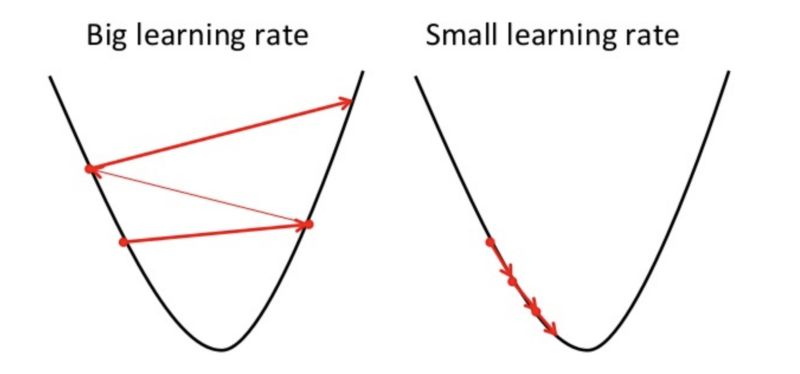
\includegraphics[width=0.7\textwidth]{Figures/Section3_learningrate.png} 
	\centering
	\caption{Influence of big and small learning rate. Too big learning rate result in bounces around the local optima, however too small value cause low efficiency }
	\label{fig:lr}
\end{figure}

There are three popular types of Gradient Descent, that mainly differ in the amount of data they use.
\begin{itemize}
	\item \textbf{Batch Gradient Descent:}
	
	Batch Gradient Descent, also called vanilla gradient descent, calculates the error for each example within the training dataset, but only after all training examples have been evaluated, the model gets updated. This whole process is like a cycle and called a training epoch.
	
	Advantages of it are that it’s computational efficient, it produces a stable error gradient and a stable convergence. Batch Gradient Descent has the disadvantage that the stable error gradient can sometimes result in a state of convergence that isn’t the best the model can achieve. It also requires that the entire training dataset is in memory and available to the algorithm \cite{goodfellow2016deep}.
	
	\item \textbf{Stochastic Gradient Descent:}
	
	Stochastic gradient descent (SGD) in contrary, does this for each training example within the dataset. This means that it updates the parameters for each training example, one by one. This can make SGD faster than Batch Gradient Descent, depending on the problem. One advantage is that the frequent updates allow us to have a pretty detailed rate of improvement. SGD can lead to "zig-zagging" behavior, where the single data point estimate of the gradient keeps changing direction and does not approach the minimum directly \cite{goodfellow2016deep}.
	
	The thing is that the frequent updates are more computationally expensive as the approach of Batch Gradient Descent. The frequency of those updates can also result in noisy gradients, which may cause the error rate to jump around, instead of slowly decreasing.
	
	\item \textbf{Mini Batch Gradient Descent:}	
	
	Mini-batch Gradient Descent is the go-to method since it’s a combination of the concepts of SGD and Batch Gradient Descent. It simply splits the training dataset into small batches and performs an update for each of these batches. Therefore it creates a balance between the robustness of stochastic gradient descent and the efficiency of batch gradient descent \cite{yang2016craft}.
	
	Common mini-batch sizes range between 50 and 256, but like for any other machine learning techniques, there is no clear rule, because they can vary for different applications. Note that it is the go-to algorithm when you are training a neural network and it is the most common type of gradient descent within deep learning.	
\end{itemize}

\begin{figure}[h]
	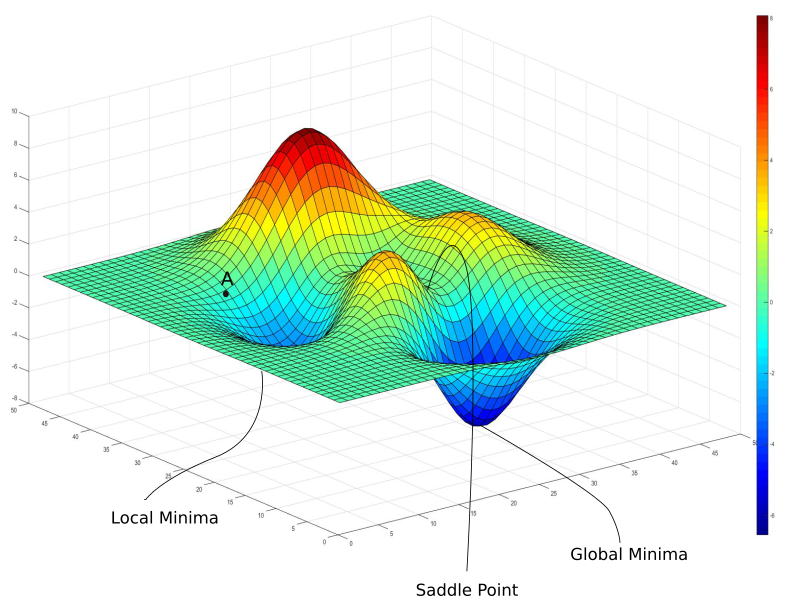
\includegraphics[width=0.7\textwidth]{Figures/Section3_GD_localminima.png} 
	\centering
	\captionsetup{justification=centering}
	\caption{Local minima and global minima}
	\label{fig:localminima}
\end{figure}

\subsubsection*{Back Propagation}
A neural network is trained by selecting the weights of all neurons so that the network learns to approximate target outputs from known inputs. It is difficult to solve the neuron weights of a multi-layer network analytically. The \textit{back-propagation algorithm} \cite{bishop2006pattern,goodfellow2016deep},provides a simple and effective solution to solving the weights iteratively. 

The backpropagation is an algorithm to propagate back the error from the loss function through the network to compute the gradient $ \frac{\partial \mathcal{L}}{\partial w_{ij}} $

In the first phase of the algorithm, an input vector is propagated forward through the neural network. Before this, the weights of the network neurons have been initialized to some values, for example small random values. The received output of the network is compared to the desired output (which should be known for the training examples) using a loss function. The gradient of the loss function is then computed. This gradient is also called the error value. When using mean squared error as the loss function, the output layer error value is simply the difference between the current and desired output.

The error values are then propagated back through the network to calculate the error values of the hidden layer neurons. The hidden neuron loss function gradients can be solved using the chain rule of derivatives. Finally, the neuron weights are updated by calculating the gradient of the weights and subtracting a proportion of the gradient from the weights, which known as gradient descent we mentioned in previous chapters. This ratio is called the \textit{learning rate} \cite{bishop2006pattern}. The learning rate can be fixed or dynamic. After the weights have been updated, the algorithm continues by executing the phases again with different input until the weights converge.

\subsection{Deep Learning and Convolutional neural networks}
\subsubsection*{Difference Between Machine Learning and Deep Learning}
Deep learning is a specialized form of machine learning. A machine learning workflow starts with relevant features being manually extracted from images. The features are then used to create a model that categorizes the objects in the image. With a deep learning workflow, relevant features are automatically extracted from images. In addition, deep learning performs “end-to-end learning” – where a network is given raw data and a task to perform, such as classification, and it learns how to do this automatically.

Another key difference is deep learning algorithms scale with data, whereas shallow learning converges. Shallow learning refers to machine learning methods that plateau at a certain level of performance when you add more examples and training data to the network.A key advantage of deep learning networks is that they often continue to improve as the size of your data increases.

\subsubsection*{Overview of Convolutional Neural Networks}
Convolution Neural Networks (ConvNets) are specialized Artificial Neural Networks. ConvNets are well suited for the processing of images, but the same concepts are adaptable for other fields, like audio or video. In this section, we describe the ConvNets for the processing of images.

A ConvNet consists of multiple convolution and pooling layers. At the end follows normally a fully connected layer. A pooling layer is applied after one or multiple convolution layers. The convolution layers have the task to extract useful features from the input, which results in multiple feature maps. The pooling layer reduces the spatial size of these feature maps.

\subsubsection*{Convolution layer}
A convolution layer consists of units as well as a normal neural network, but with a different arrangement and a different connectionism of the units. The main differences to the neural networks are:
 A convolution layer consists of units as well as a normal neural network, but with a different arrangement and a different connectionism of the units. The main differences to the neural networks are:
	\begin{itemize}
		\item Three dimensional arrangement of the unit, instead of 1 dimension
		\item Weight sharing
		\item Local connectivity
	\end{itemize}

The three dimensional arrangement comes from the image. A colored image has normally three channels (red, green, blue), and every channel is described by a two dimensional matrix. Therefore, the input of the ConvNet is a three dimensional matrix. The output of a convolution layer is again a three dimensional matrix, with feature maps of two dimensions and this x times for the number of filters for this layer. Every filter produces a feature map. 

\textbf{Weight sharing} means that the same weights are used for multiple output units.  Through this, the ConvNet gets the property, that the features are invariant against translation. This means, that a feature can be found on the complete input. To compare this with the Sobel filter, the weights are the filter, and this filter will be used on the complete input to generate the output.

\textbf{Local connectivity} means that that not all units of the input are connected with the output unit. The size of the local connectivity is described by the kernel size.

In the Convolutional layers image can be filtered using the convolution operation \cite{marr1980theory}. A convolution kernel, or filter, describes how each pixel will be influenced by its neighbors. For example, a blurring filter will take the weighted average of neighboring pixels so that large differences between pixel values are reduced. By using the same source image and changing only the filter, one can produce effects such as sharpening, blurring, edge enhancing, and embossing.

Convolution algorithms works by iterating over each pixel in the source image. For each source pixel, the filter is centered over the pixel, and the values of the filter multiply the pixel values that they overlay. A sum of the products is then taken to produce a new pixel value. Figure 3.14 provides a visual representation for this algorithm. 
\begin{figure}[h]
	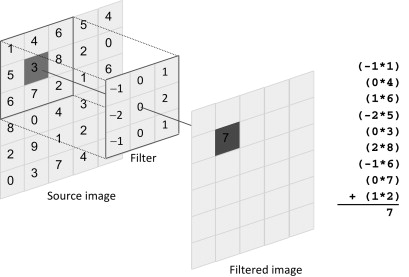
\includegraphics[width=0.7\textwidth]{Figures/Section3_Convfilter.jpg} 
	\centering
	\caption{Convolution filter}
	\label{fig:Convfilter}
\end{figure}

The discrete convolution operation between an image f and a filter matrix g is defined as:

\begin{equation}
	h[x,y]=f[x,y]*g[x,y]=\sum_{n}\sum_{m} f[n,m]g[x-n][y-m]
\end{equation}

In effect, the dot product of the filter g and a sub-image of f (with same dimensions as g) centred on coordinates x, y produces the pixel value of h at coordinates x, y \cite{goodfellow2016deep}.  The size of the receptive field is adjusted by the size of the filter matrix. Aligning the filter successively with every sub-image of f produces the of output pixel matrix h. In the case of neural networks, the output matrix is also called an feature map \cite{goodfellow2016deep}(or an activation map after computing the activation function). Edges need to be treated as a special case. If image f is not padded, the output size decreases slightly with every convolution.

A set of convolutional filters can be combined to form a \textit{convolutional layer} of a neural network \cite{fukushima1988neocognitron}. The matrix values of the filters are treated as neuron parameters and trained using machine learning. The convolution operation replaces the multiplication operation of a regular neural network layer. Output of the layer is usually described as a volume. The height and width of the volume depend on the dimensions of the activation map. The depth of the volume depends on the number of filters.

Since the same filters are used for all parts of the image, the number of free parameters is reduced drastically compared to a fully-connected neural layer \cite{lecun1989backpropagation}.  The neurons of the convolutional layer mostly share the same parameters and are only connected to a local region of the input. Parameter sharing resulting from convolution ensures translation invariance. An alternative way of describing the convolutional layer is to imagine a fully-connected layer with an infinitely strong prior placed on its weights \cite{goodfellow2016deep}. This prior forces the neurons to share weights at different spatial locations and to have zero weight outside the receptive field.

\begin{figure}[h]
	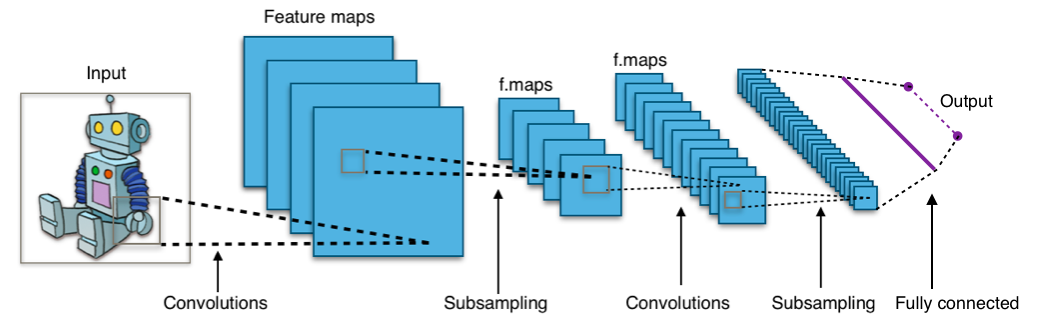
\includegraphics[width=\textwidth]{Figures/Section3_Convnetwork.png} 
	\centering
	\captionsetup{justification=centering}
	\caption{An example of a convolutional network}
	\label{fig:Convnetwork}
\end{figure}

Successive convolutional layers (often combined with other types of layers, such as pooling described below) form a \textit{convolutional neural network}(CNN).  An example of a convolutional network is shown in figure 3.15. The back-propagation training algorithm, described in previous section, is also applicable to convolutional networks \cite{goodfellow2016deep}.  In theory, the layers closer to the input should learn to recognize low-level features of the image, such as edges and corners, and the layers closer to the output should learn to combine these features to recognize more meaningful shapes \cite{fukushima1988neocognitron}.

\subsubsection*{Pooling and stride}
The pooling layer is normally applied after some convolution layers. It has the function to reduce the spatial size of the feature maps. This reduce the amount of parameters and the computation time, because the next layer get a smaller version of the feature maps. In other words, it down samples the feature maps. With one pooling with the stride size of 2×2, the spatial dimension of the feature maps is reduced of 75\%. The pooling works independently on every feature map and has no activation function or weights to learn. Furthermore, the pooling layer helps to be invariant to small translations of the input, because a small translation has mostly no change on the values of the outputs of the pooling layer.

The most common pooling layers are the max- and average-pooling. Both pooling layers take as hyperparameters the filter size and the stride. The max-pooling computes the maximum, which lies in the receptive field of the filter, and the average-pooling computes the average. An example for both poolings are depicted in figure 3.16. As recommend values for the filter size and the stride are usually for both the size of 2×2. A stride of 1×1 has no down sampling character, and therefore it is not common. A higher size for the stride has normally a negative effect, because the reduction is to much (the filter size has at the minimum the same size like the stride). A filter size of 3×3 and a stride of 2×2 has sometimes a performance gain \cite{krizhevsky2012imagenet}.

\begin{figure}[h]
	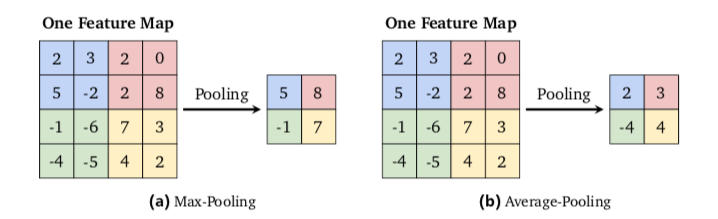
\includegraphics[width=\textwidth]{Figures/Section3_Poolinglayers.png} 
	\centering
	\captionsetup{justification=centering}
	\caption{Example for the max-pooling and the average pooling with a filter size of $2\times2$  from the Stanfrod Lecture CS231n \cite{li2015cs231n}}
	\label{fig:poolinglayer}
\end{figure}

If the feature map is not divisible by the stride without remainder, then it will be cut off the last row or column, and we lost information. In this case, it is better to add a padding. Another approach to avoid this problem is to use an input size of power of two for the network. And add to all convolutions a padding. So will be all feature maps divisible by the stride size, if the stride was 2×2.

There are further approaches for the pooling, like to use a pooling with max+average. Another approach is to use no pooling, and instead to use a convolution with a stride \cite{springenberg2014striving}. This reduce also the size of the feature maps, and has the benefit, that a further non-linearity is used.



\subsubsection*{Additional layers}
The convolutional layer typically includes a non-linear activation function, such as a rectified linear activation function. Activations are sometimes described as a separate layer between the convolutional layer and the pooling layer.

Some systems, such as \cite{simonyan2014very}, also implement a layer called local response normalization, which is used as a regularization technique. Local response normalization mimics a function of biological neurons called lateral inhibition, which causes excited neurons to decrease the activity of neighboring neurons. However, other regularization techniques are currently more popular and these are discussed in the next section.

The final hidden layers of a CNN are typically fully-connected layers \cite{bishop2006pattern}. A fully-connected layer can capture some interesting relationships parameter-sharing convolutional layers cannot. However, a fully-connected layer requires a sufficiently small data volume size in order to be practical. Pooling and stride settings can be used to reduce the size of the data volume that reaches the fully-connected layers. A convolutional network that does not include any fully-connected layers, is called a \textit{fully convolutional network}(FCN) \cite{ren2015faster}.

If the network is used for classification, it usually includes a softmax output layer \cite{bishop2006pattern}, The activations of the topmost layers can also be used directly to generate a feature representation of an image. This means that the convolutional network is used as a large feature detector \cite{lecun1989backpropagation}.

\subsubsection*{Prevent Overfitting}
A classifier trains a model which predicts the training set labels well, but fails to generalize the problem
at hand well enough to predict the labels of the test setwith satisfactory accuracy. This
phenomenon is called overfitting \cite{bishop2006pattern}.

\textbf{Data augmentation}

Overfitting can be reduced by increasing the amount of training data. When it is not possible to acquire more actual samples, data augmentation is used to generate more samples from the existing data \cite{goodfellow2016deep}.  For classification using convolutional networks, this can be achieved by computing transformations of the input images that do not alter the perceived object classes, yet provide additional challenge to the system. The images can be, for example, flipped, rotated or subsampled with different crops and scales. Also, noise can be added to the input images \cite{goodfellow2016deep}.

\textbf{Batch Normalization}

The training of a network changes the weights on every layer. This change has the effect, that the input distribution changes during updates of previously layers. The authors of batch normalization \cite{ioffe2015batch} this effect internal covariate shift. To counteract the change of the distribution during the learning, they introduced the batch normalization. Every mini-batch, which is inserted in the network, will be on every layer normalized on the input of the previously layer. The formula for the normalization is the following
\begin{align}
	\mu &\leftarrow \frac{1}{m} \sum_{i=1}^{m}x_i \\
	\sigma ^{2}&\leftarrow \frac{1}{m} \sum_{i=1}^{m}\left ( x_i-\mu  \right ) \\
	\tilde{x}&\leftarrow \frac{x_i-\mu}{\sqrt{\sigma ^{2}+\epsilon }}
\end{align}

where $\mu$ and $\sigma$ describe the mean and the standard deviation, $ \tilde{x_{i}} $ is the normalized value of the input. The value m describe the size of the mini-batch. The value $ \tilde{x} $ has then a mean of 0 and a standard deviation of 1. The batch normalization will be applied after the linear combination of a unit. The value $ \tilde{x} $ will be scaled and shifted.

At test time, $ \mu $ and $\sigma$ are replaced with the average, which is collected during the training. So it is possible to predict a single example, without to have a minibatch.

Through the applying of batch normalization, the learning rate can be increased, and this results in a faster training. Furthermore, the accuracy is increasing compared to the same network without batch normalization \cite{ioffe2015batch}.The batch normalization helps the activation function ReLU to learn faster and have a better performance \cite{ioffe2015batch}.

\textbf{Dropout}
\begin{figure}[h]
	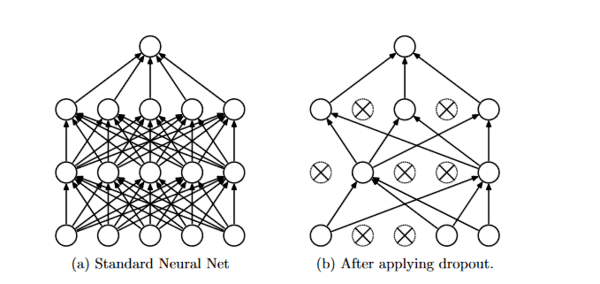
\includegraphics[width=\textwidth]{Figures/Section3_Dropout.png} 
	\centering
	\caption{Neural network with dropout  \textit{Left:}A standard neural network with 2 hidden layers. \textit{Right:}An example of a thinned net produced by applying dropout to the network \cite{srivastava2014dropout}}
	\label{fig:dropout}
\end{figure}

In CNNs or more generally machine learning overfitting is a syndrome, that hinders a model from showing generalized behavior. In simple terms the model performs good only on the training data-set, with which it is trained. Dropout is a technique for addressing this problem \cite{srivastava2014dropout}.  The key idea is to randomly drop units from the neural network during training. This prevents nodes from co-adapting too much and being dependent on
other nodes. This causes the system not to depend too much on any single neuron or connection and provides an effective yet computationally inexpensive way of implementing regularization \cite{goodfellow2016deep}.  In convolutional networks, dropout is typically used in the final fully-connected layers \cite{simonyan2014very}.  A neural network with dropout is shown in figure 3.17.


\section{Famous Network Models in field of Computer Vision}
Several designs of CNN architectures have already been created, some of them will be described here.
\subsection{VGGNet}
The VGG network architecture was introduced by Simonyan and Zisserman in their 2014 paper, \textit{Very Deep Convolutional Networks for Large Scale Image Recognition.} \cite{simonyan2014very}. It makes the improvement over AlexNet by replacing large kernel-sized filters with multiple 3×3 kernel-sized filters one after another. \\
The architecture depicted in figure 3.18 is VGG16.
\begin{figure}[h]
	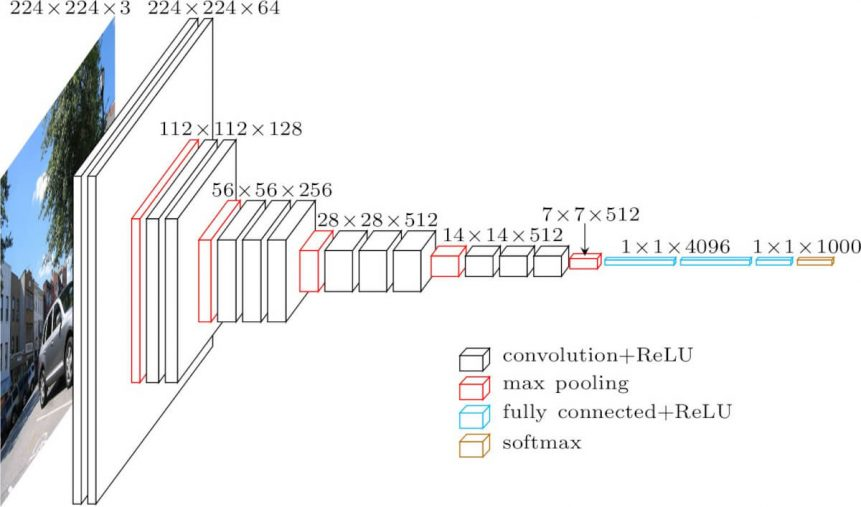
\includegraphics[width=0.7\textwidth]{Figures/Section3_Vgg16.jpg} 
	\centering
	\captionsetup{justification=centering}
	\caption{VGG-16 Architecture}
	\label{fig:vgg16}
\end{figure}
The input to cov1 layer is of fixed size 224 x 224 RGB image. The image is passed through a stack of convolutional (conv.) layers, where the filters were used with a very small receptive field: 3×3 (which is the smallest size to capture the notion of left/right, up/down, center). In one of the configurations, it also utilizes 1×1 convolution filters, which can be seen as a linear transformation of the input channels (followed by non-linearity). The convolution stride is fixed to 1 pixel; the spatial padding of conv. layer input is such that the spatial resolution is preserved after convolution, i.e. the padding is 1-pixel for 3×3 conv. layers. Spatial pooling is carried out by five max-pooling layers, which follow some of the conv.  layers (not all the conv. layers are followed by max-pooling). Max-pooling is performed over a 2×2 pixel window, with stride 2.

Three Fully-Connected (FC) layers follow a stack of convolutional layers (which has a different depth in different architectures): the first two have 4096 channels each, the third performs 1000-way ILSVRC classification and thus contains 1000 channels (one for each class). The final layer is the soft-max layer. The configuration of the fully connected layers is the same in all networks.

All hidden layers are equipped with the rectification (ReLU) non-linearity. It is also noted that none of the networks (except for one) contain Local Response Normalisation (LRN), such normalization does not improve the performance on the ILSVRC dataset, but leads to increased memory consumption and computation time.

\subsection{GoogLeNet/Inception}
The \textit{Inception} micro-architecture was first introduced by Szegedy et al. in their 2014 paper, \textit{Going Deeper with Convolutions} \cite{szegedy2015going}

While VGG achieves a phenomenal accuracy on ImageNet dataset, its deployment on even the most modest sized GPUs is a problem because of huge computational requirements, both in terms of memory and time. It becomes inefficient due to large width of convolutional layers.

In a convolutional operation at one location, every output channel is connected to every input channel, and so it can be called a dense connection architecture. The Inception architecture builds on the idea that most of the activations in a deep network are either unnecessary(value of zero) or redundant because of correlations between them. Therefore the most efficient architecture of a deep network will have a sparse connection between the activations, which implies that all output channels will not have a connection with all the input channels.

So GoogLeNet devised a module called inception module that approximates a sparse CNN with a normal dense construction, which is shown in figure 3.19. Since only a small number of neurons are effective as mentioned earlier, the width/number of the convolutional filters of a particular kernel size is kept small. Also, it uses convolutions of different sizes to capture details at varied scales. Another salient point about the module is that it has a so-called bottleneck layer(1X1 convolutions in the figure). It helps in the massive reduction of the computation requirement as explained below.
\begin{figure}[h]
	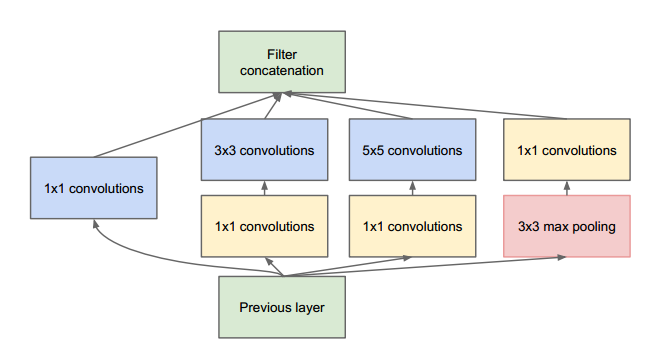
\includegraphics[width=0.7\textwidth]{Figures/Section3_Inception.png} 
	\centering
	\captionsetup{justification=centering}
	\caption{Inception module with dimension reductions}
	\label{fig:inception}
\end{figure}
Another change that GoogLeNet made, was to replace the fully-connected layers at the end with a simple global average pooling which averages out the channel values across the 2D feature map, after the last convolutional layer. This drastically reduces the total number of parameters. This can be understood from AlexNet, where FC layers contain approx. 90\% of parameters. Use of a large network width and depth allows GoogLeNet to remove the FC layers without affecting the accuracy.

\subsection{Residual Networks}
During each iteration of training a neural network, all weights receive an update proportional to the partial derivative of the error function with respect to the current weight. If the gradient is very small then the weights will not be change effectively and it may completely stop the neural network from further training. The phenomenon is called vanishing gradients  \cite{hochreiter1998vanishing}.

To overcome this problem, Microsoft introduced a deep residual learning framework \cite{he2016deep}. Instead of hoping every few stacked layers directly fit a desired underlying mapping, they explicitly let these layers fit a residual mapping. The formulation of $F(x)+x$ can be realized by feedforward neural networks with shortcut connections. Shortcut connections are those skipping one or more layers shown in figure 3.20. The shortcut connections perform identity mapping, and their outputs are added to the outputs of the stacked layers. By using the residual network, there are many problems which can be solved such as:
\begin{itemize}
	\item ResNets are easy to optimize, but the “plain” networks (that simply stack layers) shows higher training error when the depth increases.
	\item ResNets can easily gain accuracy from greatly increased depth, producing results which are better than previous networks.
\end{itemize}

\begin{figure}[h]
	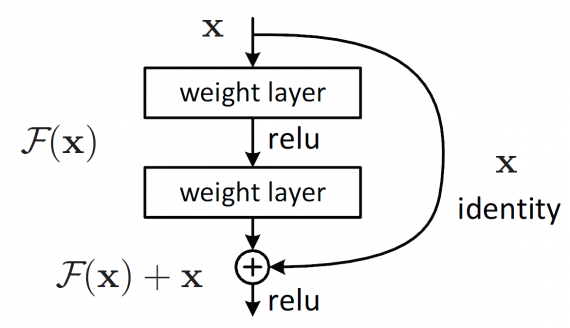
\includegraphics[width=0.7\textwidth]{Figures/Section3_Shortcut.png} 
	\centering
	\captionsetup{justification=centering}
	\caption{Shortcut connection}
	\label{fig:shortcut}
\end{figure}

Residual network \cite{he2016deep} based on the above plain network, a shortcut connection is inserted which turn the network into its counterpart residual version.  The identity shortcuts $F(x{W}+x)$ can be directly used when the input and output are of the same dimensions. When the dimensions increase, it considers two options:
\begin{itemize}
	\item The shortcut performs identity mapping, with extra zero entries padded for increasing dimensions. This option introduces no additional parameter.
	\item The projection shortcut in $F(x{W}+x)$ is used to match dimensions (done by 1×1convolutions).
\end{itemize}
For either of the options, if the shortcuts go across feature maps of two size, it performed with a stride of 2.

\begin{figure}[h]
	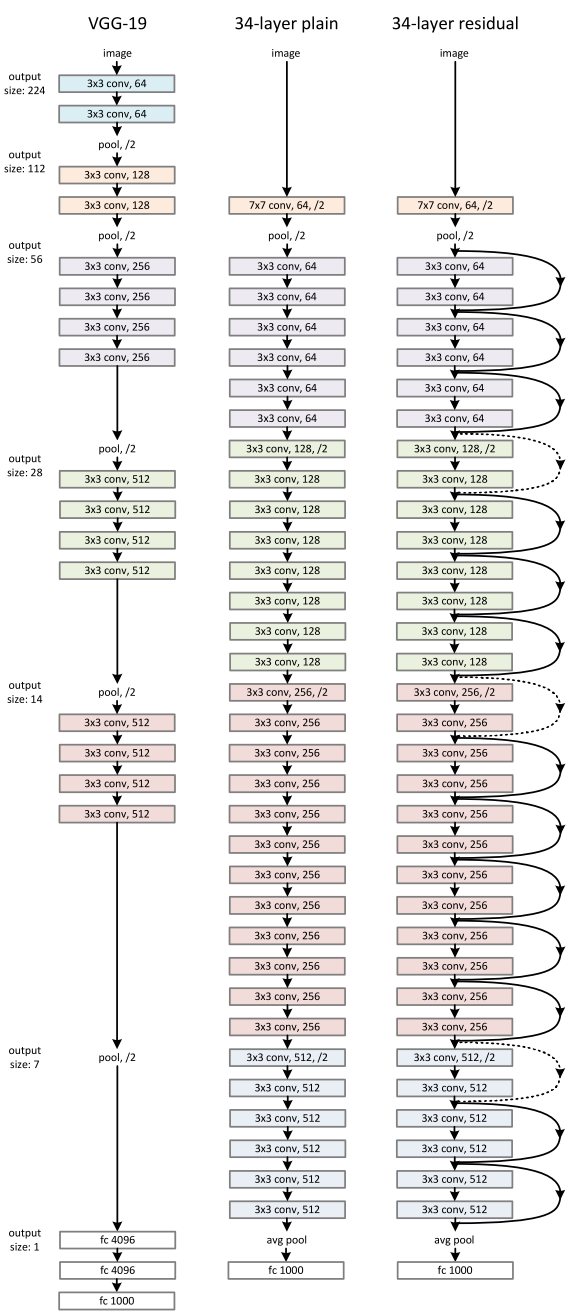
\includegraphics[width=0.6\textwidth, height=0.65\textheight]{Figures/Section3_Resnet.png} 
	\centering
	\caption{Example network architectures for ImageNet. Bottom: the
		VGG-19 model \cite{simonyan2014very} (19.6 billion FLOPs) as a reference. Middle: a plain network with 34 parameter layers (3.6 billion FLOPs). Top: a residual network with 34 parameter layers (3.6 billion FLOPs). The dotted shortcuts increase dimensions. Table 1 shows more details and other variants \cite{he2016deep}.}
	\label{fig:resnet}
\end{figure}
Even though ResNet is much deeper than VGG16 and VGG19, the model size is actually substantially smaller due to the usage of global average pooling rather than fully-connected layers.